\documentclass[11pt, letterpaper]{article}\usepackage[]{graphicx}\usepackage[]{color}
% maxwidth is the original width if it is less than linewidth
% otherwise use linewidth (to make sure the graphics do not exceed the margin)
\makeatletter
\def\maxwidth{ %
  \ifdim\Gin@nat@width>\linewidth
    \linewidth
  \else
    \Gin@nat@width
  \fi
}
\makeatother

\definecolor{fgcolor}{rgb}{0.345, 0.345, 0.345}
\newcommand{\hlnum}[1]{\textcolor[rgb]{0.686,0.059,0.569}{#1}}%
\newcommand{\hlstr}[1]{\textcolor[rgb]{0.192,0.494,0.8}{#1}}%
\newcommand{\hlcom}[1]{\textcolor[rgb]{0.678,0.584,0.686}{\textit{#1}}}%
\newcommand{\hlopt}[1]{\textcolor[rgb]{0,0,0}{#1}}%
\newcommand{\hlstd}[1]{\textcolor[rgb]{0.345,0.345,0.345}{#1}}%
\newcommand{\hlkwa}[1]{\textcolor[rgb]{0.161,0.373,0.58}{\textbf{#1}}}%
\newcommand{\hlkwb}[1]{\textcolor[rgb]{0.69,0.353,0.396}{#1}}%
\newcommand{\hlkwc}[1]{\textcolor[rgb]{0.333,0.667,0.333}{#1}}%
\newcommand{\hlkwd}[1]{\textcolor[rgb]{0.737,0.353,0.396}{\textbf{#1}}}%
\let\hlipl\hlkwb

\usepackage{framed}
\makeatletter
\newenvironment{kframe}{%
 \def\at@end@of@kframe{}%
 \ifinner\ifhmode%
  \def\at@end@of@kframe{\end{minipage}}%
  \begin{minipage}{\columnwidth}%
 \fi\fi%
 \def\FrameCommand##1{\hskip\@totalleftmargin \hskip-\fboxsep
 \colorbox{shadecolor}{##1}\hskip-\fboxsep
     % There is no \\@totalrightmargin, so:
     \hskip-\linewidth \hskip-\@totalleftmargin \hskip\columnwidth}%
 \MakeFramed {\advance\hsize-\width
   \@totalleftmargin\z@ \linewidth\hsize
   \@setminipage}}%
 {\par\unskip\endMakeFramed%
 \at@end@of@kframe}
\makeatother

\definecolor{shadecolor}{rgb}{.97, .97, .97}
\definecolor{messagecolor}{rgb}{0, 0, 0}
\definecolor{warningcolor}{rgb}{1, 0, 1}
\definecolor{errorcolor}{rgb}{1, 0, 0}
\newenvironment{knitrout}{}{} % an empty environment to be redefined in TeX

\usepackage{alltt}
\usepackage[utf8]{inputenc}
\usepackage{amsmath}
\usepackage{xcolor}
\usepackage{geometry}
\usepackage[parfill]{parskip}
\usepackage{float}
\usepackage{graphicx}
\usepackage{fancyhdr}
\graphicspath{ {.} }
\newcommand{\vv}[1]{\textcolor{black}{\mathbf{#1}}}
\definecolor{econgreen}{RGB}{55, 91, 1}

\geometry{left=2.6cm, right = 2.6cm, top = 3cm, bottom = 3cm}

\fancypagestyle{plain}{
	\let\oldheadrule\headrule% Copy \headrule into \oldheadrule
	\renewcommand{\headrule}{\color{econgreen}\oldheadrule}
	\lhead{\small{\textcolor{black}{\leftmark}}}
	%\chead{}
	\rhead{\small{\textcolor{black}{\thepage}}}
	\lfoot{}
	\cfoot{}
	\rfoot{}
	\renewcommand{\headrulewidth}{0.5pt}
	%\renewcommand{\footrulewidth}{0.5pt}
}\pagestyle{plain}
\IfFileExists{upquote.sty}{\usepackage{upquote}}{}
\begin{document}
%%%%%%%%%%%%%%%%%%%%%%%%%%%%%%%%%%%%%%%%%%%%%%%%%%%%%%%%%%%%%%%%%%%%%
\begin{titlepage}
\thispagestyle{empty}
\newgeometry{left=5cm, top=5cm} %defines the geometry for the titlepage
\pagecolor{econgreen}
\noindent

\includegraphics[width=2cm]{cmefi_short.png} \\[-1em]
\color{white}
\makebox[0pt][l]{\rule{1.3\textwidth}{1pt}}
\par
\noindent
%\textbf{\textsf{A Macroeconomic Nowcasting Model}} 
%\vskip5cm
{\Huge \textsf{A Macroeconomic Nowcasting Model}}
\vskip\baselineskip
\noindent
\textsf{March 2021}\\
\textsf{Charles Ye}
\restoregeometry % restores the geometry
\nopagecolor% Use this to restore the color pages to white
\end{titlepage}
%%%%%%%%%%%%%%%%%%%%%%%%%%%%%%%%%%%%%%%%%%%%%%%%%%%%%%%%%%%%%%%%%%%%%%





\section{Motivation}
\textbf{Nowcasting} is the prediction of the present, the near future, and the near past. Nowcasting is important in economics because many important macroeconomic statistics are released with a lengthy delay. For example, the Bureau of Economic Analysis releases quarterly GDP typically two months after the quarter has already ended - a significant delay for any companies or individuals who need the data for planning and forecast models.

This delay is particularly salient during times of high volatility. During the first few months of the COVID-19 pandemic in the United States, many companies attempted to use high-frequency indicators to attempt nowcasts of the state of the macroeconomy. For example, JP Morgan forecasts in March 13 predicted Q2 GDP growth of -3\%; the estimate was revised down to -14\% by March 21, -25\% by March 25, and -40\% by April 10. Yet many of the models were ad-hoc and only able to use a small number of predictive indicators, such as jobless claims or traffic data.

\textbf{Nowcasting is about deciphering key information about the state of the economy before official data is released.} Because of the fundamentally urgent nature of nowcasting, it is important that nowcast models exploit any latest, high-frequency data available. Nowcasts should be able to generate constantly rolling forecasts, updating these numbers in response to any new data releases.




For example, suppose the date is early March, and the variable we want to predict is Q1 GDP. The simplest way to predict Q1 GDP would be to use historical quarterly data from various economic variables. But this data would only be up to Q4 of last year, and would fail to capture the critically important predictive power that could be provided by monthly and daily data released throughout January and February.

Suppose instead, we used monthly data as our predictors of Q1 GDP. Again, we will soon run in to a problem. As an example, imagine that we had imported 20 monthly data series. Suppose 5 of these series ended in December, 10 ended in January, and 5 ended in March. 

\begin{figure}[H]
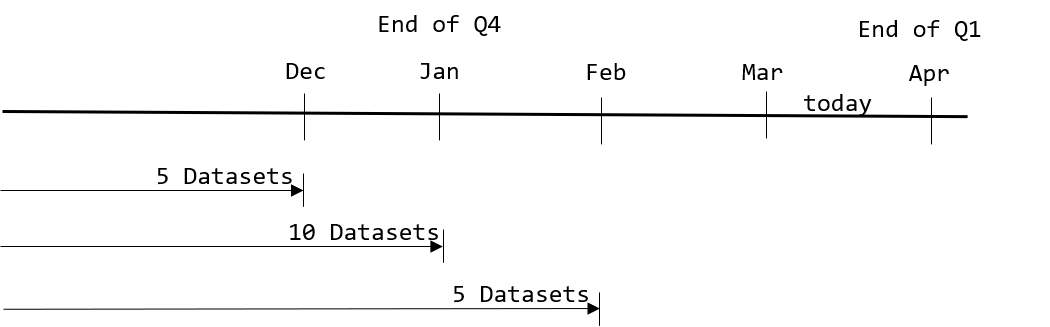
\includegraphics[scale=.7]{nowcast-time-2}
\centering
\end{figure}

Traditional modeling methods would require us to either throw out variables or throw out months - for example, we could truncate all our data series at January and lose out the information provided by the 5 February data points. Alternatively, we could completely remove the 15 variables with data releasing before March. Both methods are unappealing.

In this paper, we will utilize a methodology that will allow us to use the information from all variables at any dates. This model will give an updated forecast in response to any new data releases. Additionally, the model can be generalized to nowcast any time series variable, not just GDP. The methodology for the model will be described in the next section.
\section{Methodology}

\subsection{Overview}
This paper utilizes a modified version of the two-step dynamic factor model utilized in Giannone et al (2008) and Doz et al (2011). In this model, we use principal components to extract a few fundamental factors describing the overall structure of the economy. These factors are then projected into the future using a vector autoregression; smoothing over missing input data is conducted by using the Kalman filter and smoother. Finally, we use a formula to 

\subsection{Data}
We begin by importing monthly data from the St. Louis Federal Reserve Database (FRED). We choose data of at least monthly frequency and with historical data available as of at least 2010. Data are transformed for stationarity as listed below; \textit{dlog} refers to the natural log of the first difference.

% latex table generated in R 4.0.4 by xtable 1.8-4 package
% Fri Feb 26 20:27:59 2021
\begin{table}[!h]
\centering
\begingroup\scriptsize
\begin{tabular}{ll}
  \hline
Variable & Stationary Form \\ 
  \hline
PCE & dlog \\ 
  PCE: Goods & dlog \\ 
  PCE: Goods: Durable Goods & dlog \\ 
  PCE: Goods: Nondurable Goods & dlog \\ 
  PCE: Services & dlog \\ 
  Disposable Personal Income & dlog \\ 
  Case-Shiller Housing Price Index & dlog \\ 
  Effective Federal Funds Rate & base \\ 
  Treasury Yield 10Y & base \\ 
  Treasury Yield 1Y & base \\ 
  Vehicle Sales & base \\ 
  Unemployment rate & dlog \\ 
  Weekly Economic Index & base \\ 
  S\&P 500 & dlog \\ 
  VIX & base \\ 
  Outstanding Real Estate Loans & dlog \\ 
  Outstanding Credit Card Balances & dlog \\ 
  St. Louis Fed Financial Stress Index & base \\ 
  U.S. Dollar Index & base \\ 
  Average Weeks Unemployed & base \\ 
  Retail \& Food Sales & dlog \\ 
  KC Fed Labor Market Index & base \\ 
  Consumer Confidence (OECD) & base \\ 
  Industrial Production index & dlog \\ 
  New York Fed: Business Conditions Manufacturing Survey & base \\ 
  Chicago Fed National Activity Index & base \\ 
   \hline
\end{tabular}
\endgroup
\caption{Imported Monthly Data} 
\end{table}


We additionally import quarterly data for GDP and its subcomponents.
% latex table generated in R 4.0.4 by xtable 1.8-4 package
% Fri Feb 26 20:27:59 2021
\begin{table}[!h]
\centering
\begingroup\scriptsize
\begin{tabular}{ll}
  \hline
Variable & Stationary Form \\ 
  \hline
GDP & dlog \\ 
  Personal Consumption & dlog \\ 
  Personal Consumptions: Goods & dlog \\ 
  Personal Consumptions: Goods: Durable & dlog \\ 
  Personal Consumptions: Goods: Durable: Motor Vehicles \& Parts & dlog \\ 
  Personal Consumptions: Goods: Durable: Furnishings \& Durable Household Equipment & dlog \\ 
  Personal Consumptions: Goods: Durable: Recreational Goods \& Services & dlog \\ 
  Personal Consumptions: Goods: Durable: Other Durable Goods & dlog \\ 
  Personal Consumptions: Goods: Nondurable Goods & dlog \\ 
  Personal Consumptions: Goods: Nondurable Goods: Food \& Beverages for Off-Premises Consumption & dlog \\ 
  Personal Consumptions: Goods: Nondurable Goods: Clothing & dlog \\ 
  Personal Consumptions: Goods: Nondurable Goods: Gasoline \& Energy Goods & dlog \\ 
  Personal Consumptions: Goods: Nondurable Goods: Other Nondurable Goods & dlog \\ 
  Personal Consumptions: Services & dlog \\ 
  Personal Consumptions: Services: Housing \& Utilities & dlog \\ 
  Personal Consumptions: Services: Health Care & dlog \\ 
  Personal Consumptions: Services: Transportation & dlog \\ 
  Personal Consumptions: Services: Recreation & dlog \\ 
  Personal Consumptions: Services: Food Services \& Accomodations & dlog \\ 
  Personal Consumptions: Services: Financial Services & dlog \\ 
  Personal Consumptions: Services: Other Services & dlog \\ 
  Personal Consumptions: Services: Nonprofit Services & dlog \\ 
  Gross Private Domestic Investment & dlog \\ 
  Gross Private Domestic Investment: Nonresidential Investment & dlog \\ 
  Gross Private Domestic Investment: Nonresidential Investment: Structures & dlog \\ 
  Gross Private Domestic Investment: Nonresidential Investment: Equipment & dlog \\ 
  Gross Private Domestic Investment: Nonresidential Investment: Intellectual Property & dlog \\ 
  Gross Private Domestic Investment: Residential Investment & dlog \\ 
  Gross Private Domestic Investment: Change in Private Inventories & base \\ 
  Net Exports & base \\ 
  Exports & dlog \\ 
  Exports: Goods & dlog \\ 
  Exports: Services & dlog \\ 
  Imports & dlog \\ 
  Imports: Goods & dlog \\ 
  Imports: Services & dlog \\ 
  Government consumption expenditures and gross investment & dlog \\ 
  Federal & dlog \\ 
  State and local & dlog \\ 
  Weekly Economic Index & base \\ 
  Industrial Production index & dlog \\ 
  Chicago Fed National Activity Index & base \\ 
   \hline
\end{tabular}
\endgroup
\caption{Imported Quarterly Data} 
\end{table}


Most datasets have already been deseasonalized if necessary by their original source. We deseasonalize the remaining series by using the U.S. Census Bureau's seasonal adjustment package, X13-ARIMA-SEATS. We interface with it by using the \texttt{seasonal} package implementation in R (Sax and Eddelbuettel 2018).

\subsection{Time Periods}
Now we will segment the data by time periods. The imported monthly data will have ragged edges - i.e., some monthly data will be available for later months than others.

We will let $T$ denote the number of dates for which data is available for all data series. $\tau$ will denote the number of dates for which data is available for at least one data series. $T*$ will denote number of dates up to the end-of-quarter month of the $\tau$ date. For example, suppose date $\tau$ occurs on February. The end-of-quarter month, $T^*$, will be March (since Q1 runs through the end of March). 

In other words, data will be indexed by $t = 1, 2, \dots, T, T+1, \dots, \tau, \dots, T^*$, where dates $T + 1$ through $\tau$ are the dates for which only some data are available, and dates $\tau + 1$ through $T^*$ are the dates for which no data is available up to the next quarter-ending month.
\begin{figure}[H]
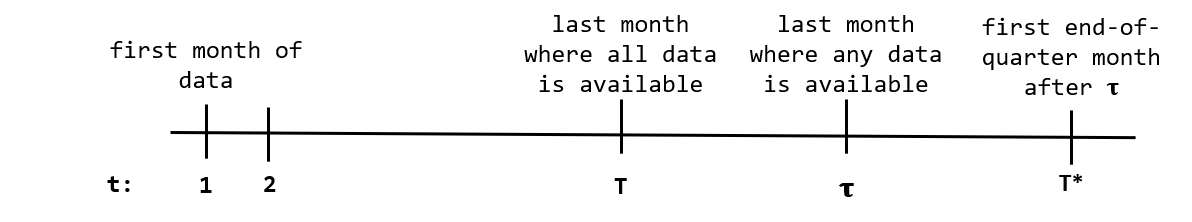
\includegraphics[scale=.7]{nowcast-time}
\centering
\end{figure}



\subsection{Principal Components Analysis}
It is known that a large number of macroeconomic time series are highly correlated; using such covariates as regressors could naturally lead to problems with collinearity and unstable estimates. In addition, it becomes computationally burdensome to analyze data with such a large number of highly correlated variables. Instead, we use principal components analysis (PCA) to shrink our dataset in a way that allows us to retain most of the information in our original data.

Estimation of factors is derived following Stock and Watson (2008). We begin by taking our $T \times N$ data matrix of $N$ monthly covariates, from time 1 through $T$. The matrix, which we denote $X$, is normalized to mean 0 and variance 0 across all columns.

The goal is to minimize the error $E$ below.
\begin{align*}
	X = F  \Lambda ' + E,\\
	\text{where $X$ is the $T \times N$ data matrix,}\\
	\text{$F$ is the $T \times N$ matrix of factors,}\\
	\text{and $\Lambda$ is the weighting matrix.}\\
\end{align*}

Estimation of factors is derived following Stock and Watson (2008).
\begin{align*}
	\widehat{\Lambda} = \text{eigenvectors of } (X'X)\\
	\widehat{F} = X \widehat{\Lambda}
\end{align*}

Once factors are derived, we perform a qualitative check of the factors. Typically the first factor should give us something similar to the growth rate of GDP or aggregate production, but on a monthly basis. The second and third factors may vary but often represent interest rates or consumption. Note that the sign direction of the factors is irrelevant to the modeling process, and they may be switched negated without consequence. 



{\centering 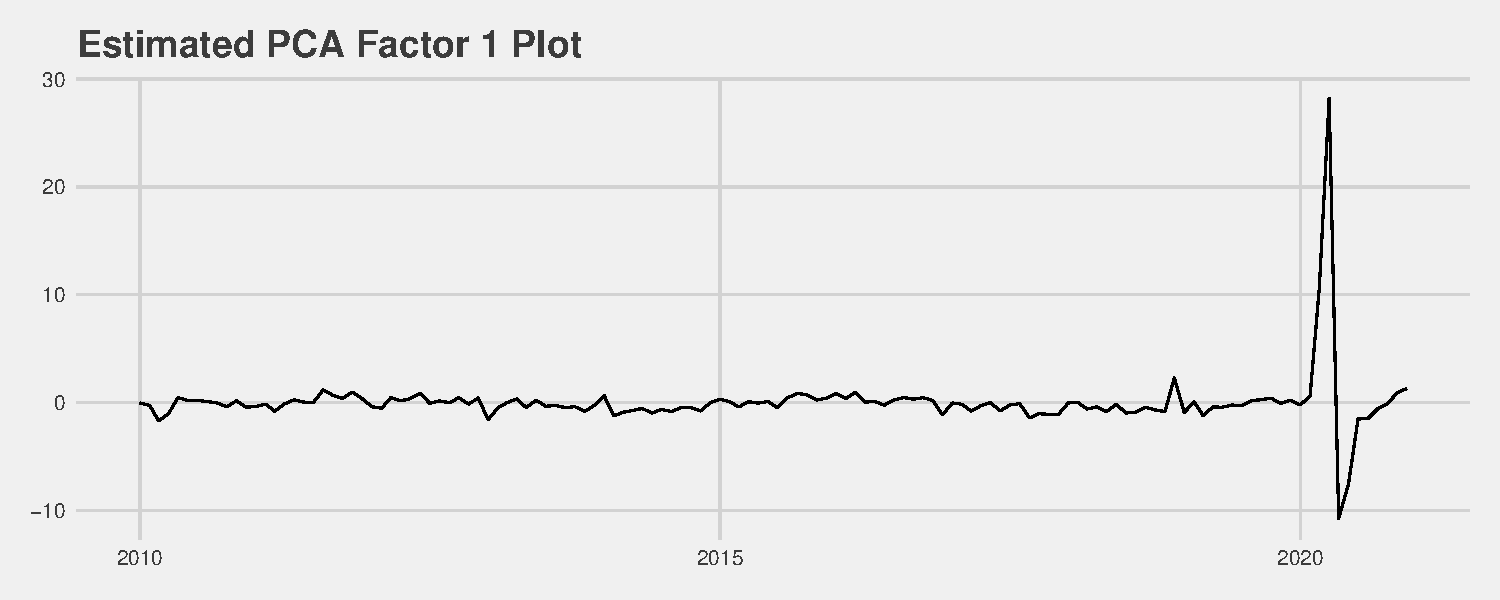
\includegraphics[width=5in,height=2in]{figure/unnamed-chunk-4-1} 

}




{\centering 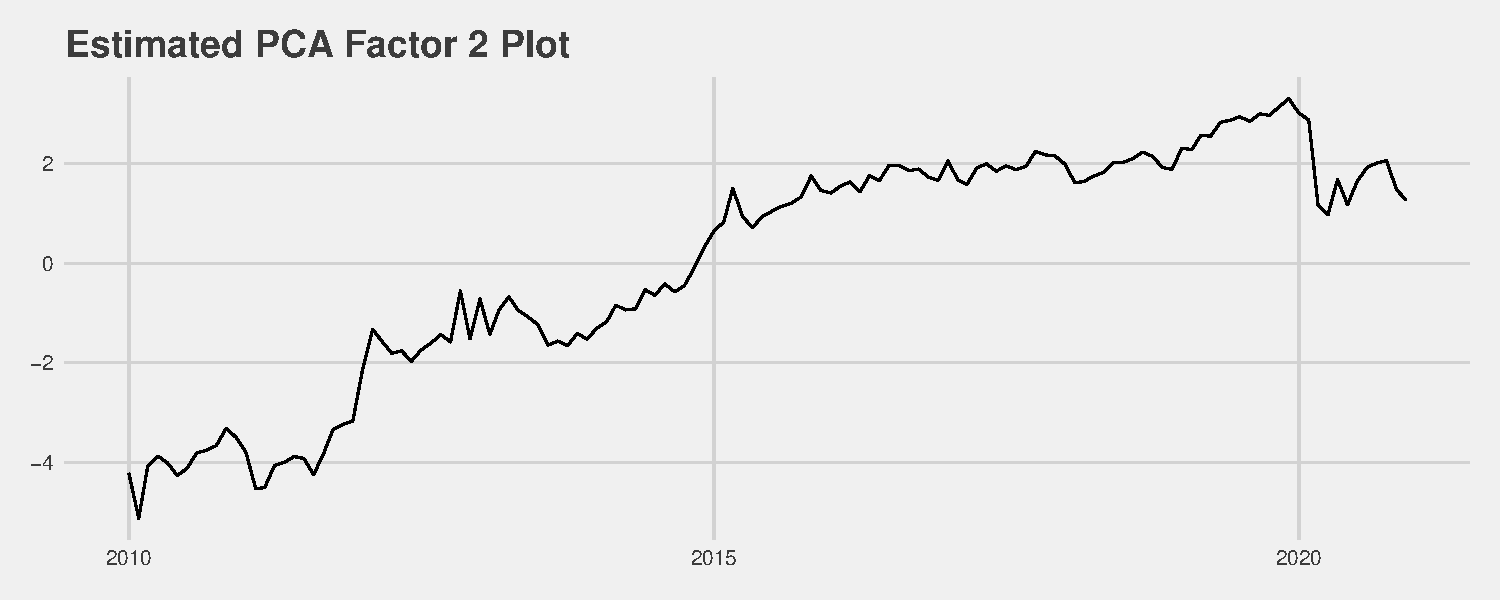
\includegraphics[width=5in,height=2in]{figure/unnamed-chunk-4-2} 

}




{\centering 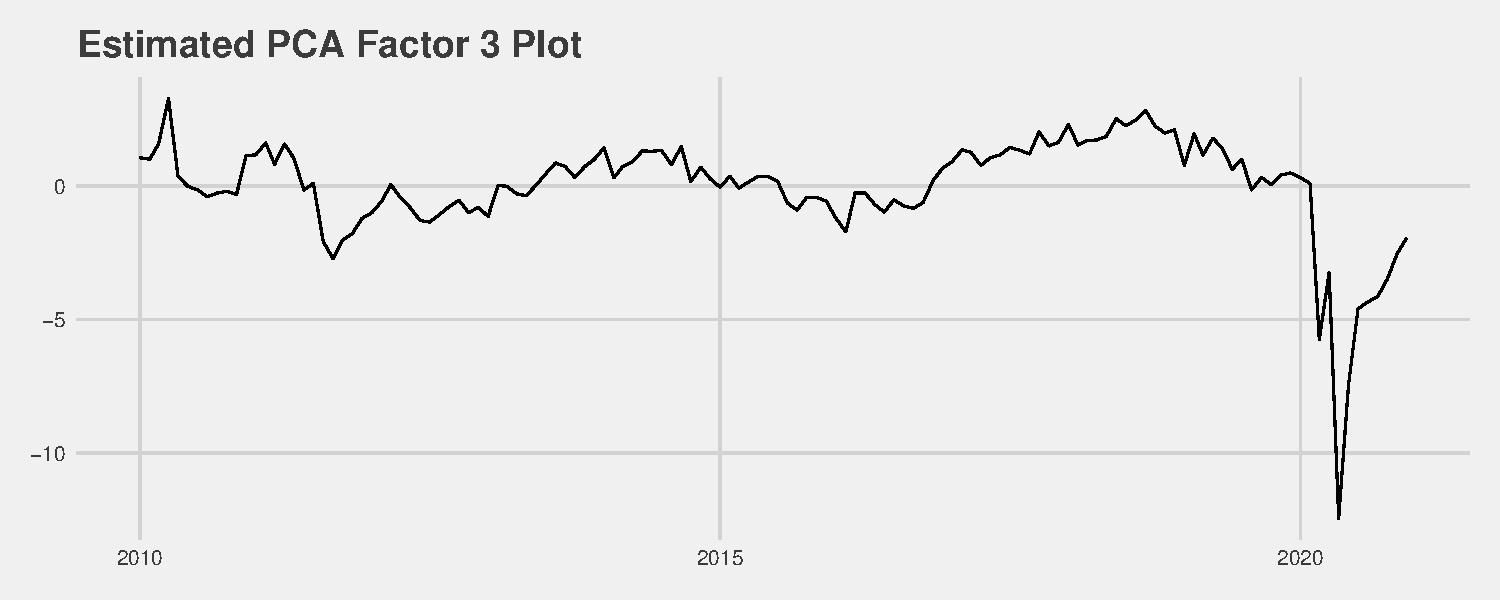
\includegraphics[width=5in,height=2in]{figure/unnamed-chunk-4-3} 

}





Once factors are derived, we select the optimal number of factors to use in predictive regressions. To do so, we use the information criteria from Bai and Ng (2002). Let $R$ refer to the number of factors used. We include alternative specifications of the information criteria from Bai and Ng as a robustness check.
\begin{align*}
	IC(R) = MSE + R \frac{N+T}{NT} log\left(\frac{NT}{N+T}\right)
\end{align*}



{\centering 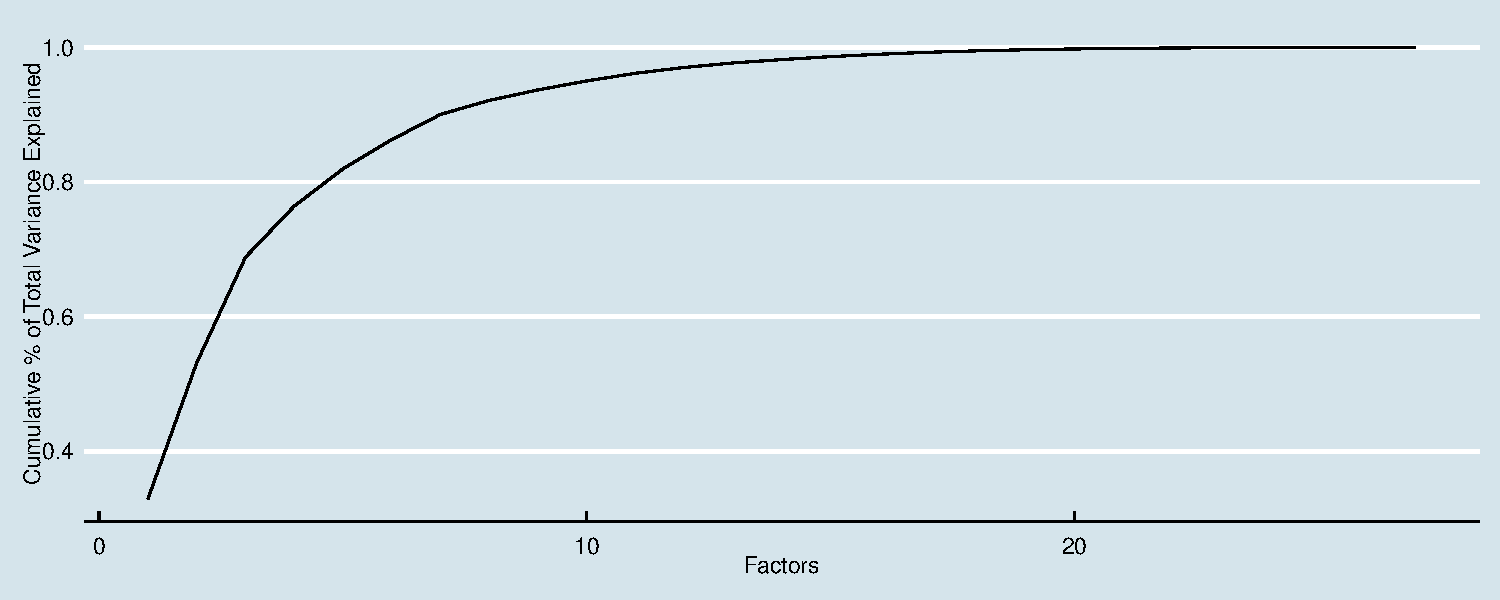
\includegraphics[width=5in,height=2in]{figure/unnamed-chunk-5-1} 

}




% latex table generated in R 4.0.4 by xtable 1.8-4 package
% Fri Feb 26 20:28:00 2021
\begin{table}[!h]
\centering
\begingroup\footnotesize
\begin{tabular}{rrrrrrrr}
  \hline
factors & var\_explained & pct\_of\_total & cum\_pct\_of\_total & mse & ic1 & ic2 & ic3 \\ 
  \hline
  1 & 8.67 & 0.33 & 0.33 & 0.66 & 0.80 & 0.81 & 0.79 \\ 
    2 & 5.46 & 0.21 & 0.54 & 0.45 & 0.74 & 0.75 & 0.70 \\ 
    3 & 3.87 & 0.15 & 0.69 & 0.31 & 0.73 & 0.76 & 0.68 \\ 
    4 & 2.03 & 0.08 & 0.77 & 0.23 & 0.79 & 0.83 & 0.73 \\ 
    5 & 1.50 & 0.06 & 0.83 & 0.17 & 0.88 & 0.92 & 0.80 \\ 
    6 & 1.05 & 0.04 & 0.87 & 0.13 & 0.98 & 1.03 & 0.88 \\ 
    7 & 0.98 & 0.04 & 0.91 & 0.09 & 1.09 & 1.14 & 0.97 \\ 
    8 & 0.56 & 0.02 & 0.93 & 0.07 & 1.21 & 1.27 & 1.07 \\ 
    9 & 0.42 & 0.02 & 0.94 & 0.06 & 1.33 & 1.41 & 1.18 \\ 
   10 & 0.32 & 0.01 & 0.96 & 0.04 & 1.46 & 1.54 & 1.30 \\ 
   11 & 0.28 & 0.01 & 0.97 & 0.03 & 1.59 & 1.68 & 1.41 \\ 
   12 & 0.21 & 0.01 & 0.97 & 0.03 & 1.73 & 1.82 & 1.53 \\ 
   13 & 0.15 & 0.01 & 0.98 & 0.02 & 1.86 & 1.97 & 1.65 \\ 
   14 & 0.13 & 0.01 & 0.99 & 0.01 & 2.00 & 2.11 & 1.77 \\ 
   15 & 0.10 & 0.00 & 0.99 & 0.01 & 2.14 & 2.26 & 1.89 \\ 
   16 & 0.08 & 0.00 & 0.99 & 0.01 & 2.27 & 2.41 & 2.01 \\ 
   17 & 0.06 & 0.00 & 0.99 & 0.01 & 2.41 & 2.56 & 2.14 \\ 
   18 & 0.04 & 0.00 & 1.00 & 0.00 & 2.55 & 2.70 & 2.26 \\ 
   19 & 0.03 & 0.00 & 1.00 & 0.00 & 2.69 & 2.85 & 2.38 \\ 
   20 & 0.02 & 0.00 & 1.00 & 0.00 & 2.84 & 3.00 & 2.51 \\ 
   21 & 0.02 & 0.00 & 1.00 & 0.00 & 2.98 & 3.15 & 2.63 \\ 
   22 & 0.01 & 0.00 & 1.00 & 0.00 & 3.12 & 3.30 & 2.76 \\ 
   23 & 0.01 & 0.00 & 1.00 & 0.00 & 3.26 & 3.45 & 2.88 \\ 
   24 & 0.00 & 0.00 & 1.00 & 0.00 & 3.40 & 3.60 & 3.01 \\ 
   25 & 0.00 & 0.00 & 1.00 & 0.00 & 3.54 & 3.75 & 3.13 \\ 
   26 & 0.00 & 0.00 & 1.00 & 0.00 & 3.68 & 3.90 & 3.26 \\ 
   \hline
\end{tabular}
\endgroup
\caption{Factor Selection Process} 
\end{table}


Choosing the IC-minimizing $R$ lets us choose $R = 3$ factors.



\subsection{Factor VAR}
The next step is to model the transition of the factors over time. To do so, we utilize a vector-autoregressive (VAR) process, following Stock and Watson (2016).
\begin{align*}
\underbrace{\begin{bmatrix}
	\vv{f1}_{t}\\
	\vv{f2}_{t}\\
	\vdots \\
	\vv{fR}_{t}
\end{bmatrix}}_{z_t}
=
B
\underbrace{\begin{bmatrix}
	\vv{f1}_{t-1}\\
	\vv{f2}_{t-1}\\
	\vdots \\
	\vv{fR}_{t-1}
\end{bmatrix}}_{z_{t-1}}
+
C
+
\underbrace{\begin{bmatrix}
v1_t\\
v2_t\\
\vdots\\
vR_t
\end{bmatrix}}_{v_t},\\
\text{where $z_t$ is the $R \times 1$ matrix of time $t$ factors,}\\
\text{$B$ is the $R \times R$ coefficient matrix,}\\
\text{$C$ is the $R \times 1$ constant matrix,}\\
\text{and $v_t$ is the $R \times 1$ matrix of errors for time $t$.}
\end{align*}


We wish to estimate the coefficient matrices $B$ and $C$. This can be done via OLS estimation. We first rewrite the data as the standard linear equation,
\begin{align*}
\underbrace{\begin{bmatrix}
\vv{f1}_{2} & \vv{f2}_{2} & \dots & \vv{f6}_{2}\\
\vv{f1}_{3} & \vv{f2}_{3} & \dots & \vv{f6}_{3}\\
\vdots & \vdots & \vdots & \vdots \\
\vv{f1}_{T} & \vv{f2}_{T} & \dots & \vv{f6}_{T}
\end{bmatrix}}_{\Gamma}
=
\underbrace{\begin{bmatrix}
1 & \vv{f1}_{1} & \vv{f2}_{1} & \dots & \vv{f6}_{1}\\
1 & \vv{f1}_{2} & \vv{f2}_{2} & \dots & \vv{f6}_{2}\\
\vdots & \vdots & \vdots & \vdots & \vdots \\
1 & \vv{f1}_{T-1} & \vv{f2}_{T-1} & \dots & \vv{f6}_{T-1}
\end{bmatrix}}_{\Psi}
\underbrace{\begin{bmatrix}
C'\\
B'
\end{bmatrix}}_{\Lambda}
 +
\underbrace{\begin{bmatrix}
v1_2 & v2_2 & \dots & vR_2\\
v1_3 & v2_3 & \dots & vR_3\\
\vdots\\
v1_T & v2_T & \dots & vR_T\\
\end{bmatrix}}_{V},\\
\text{where $\Gamma$ is the $T-1 \times R$ dependent data matrix,}\\
\text{$\Psi$ is the $T-1 \times R+1$ independent data matrix,}\\
\text{$\Lambda$ is the $R+1 \times R$ matrix of coefficient weightings,}\\
\text{and $V$ is the $T-1 \times R$ matrix of residuals.}
\end{align*}
The coefficient matrix $\Lambda$ can be estimated by the standard OLS estimator.
\begin{align*}
\widehat{\Lambda} = (\Psi' \Psi)^{-1} (\Psi'\Gamma)
\end{align*}
It can then be partitioned to calculate $\widehat{B}'$ and $\widehat{C}'$, which can then be transposed to derive our estimates of the original coefficient matrices B and C, $\widehat{B}$ and $\widehat{C}$.

The estimated coefficients in $B$ and $C$ are shown below.
% latex table generated in R 4.0.4 by xtable 1.8-4 package
% Fri Feb 26 20:28:00 2021
\begin{table}[!h]
\centering
\begingroup\footnotesize
\begin{tabular}{lrrrr}
  \hline
name & constant & f1.l1 & f2.l1 & f3.l1 \\ 
  \hline
f1 & 0.00 & 0.10 & 0.05 & -0.12 \\ 
  f2 & 0.04 & 0.02 & 0.98 & -0.00 \\ 
  f3 & -0.02 & -0.28 & 0.00 & 0.80 \\ 
   \hline
\end{tabular}
\endgroup
\caption{Factor VAR Coefficients} 
\end{table}



Finally, we perform a qualitative check of the fitted values.


{\centering 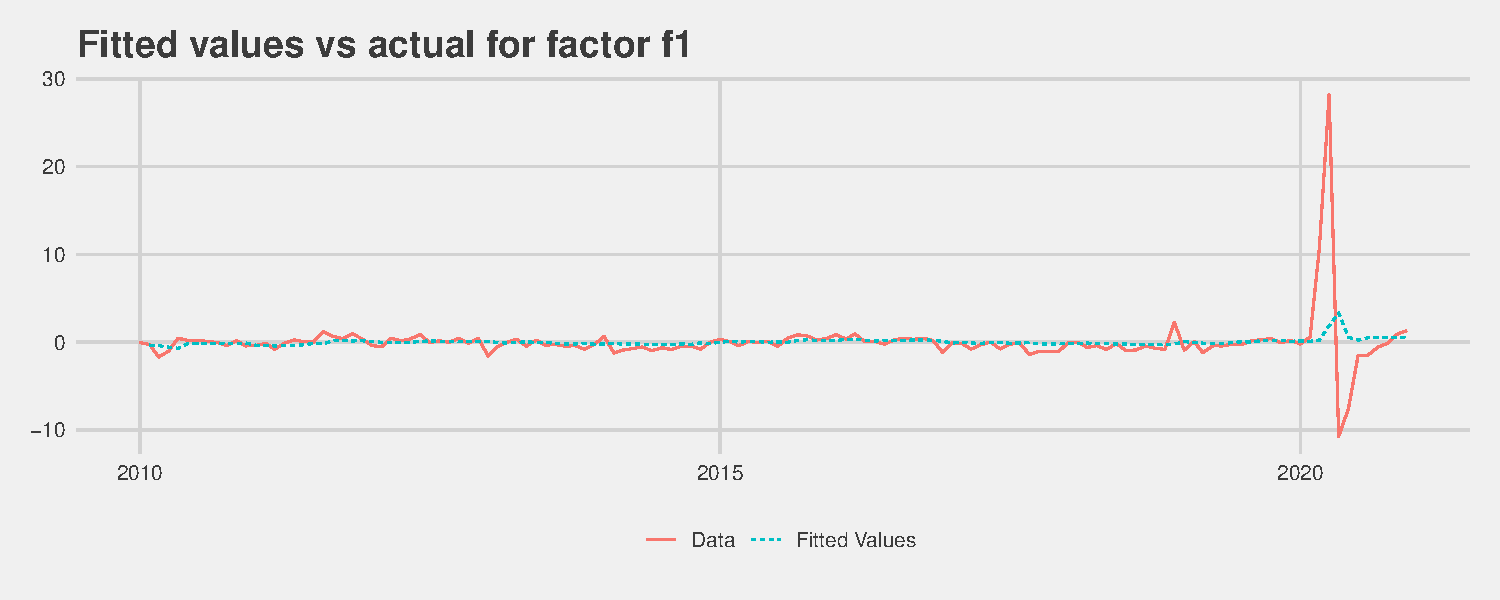
\includegraphics[width=5in,height=2in]{figure/unnamed-chunk-8-1} 

}




{\centering 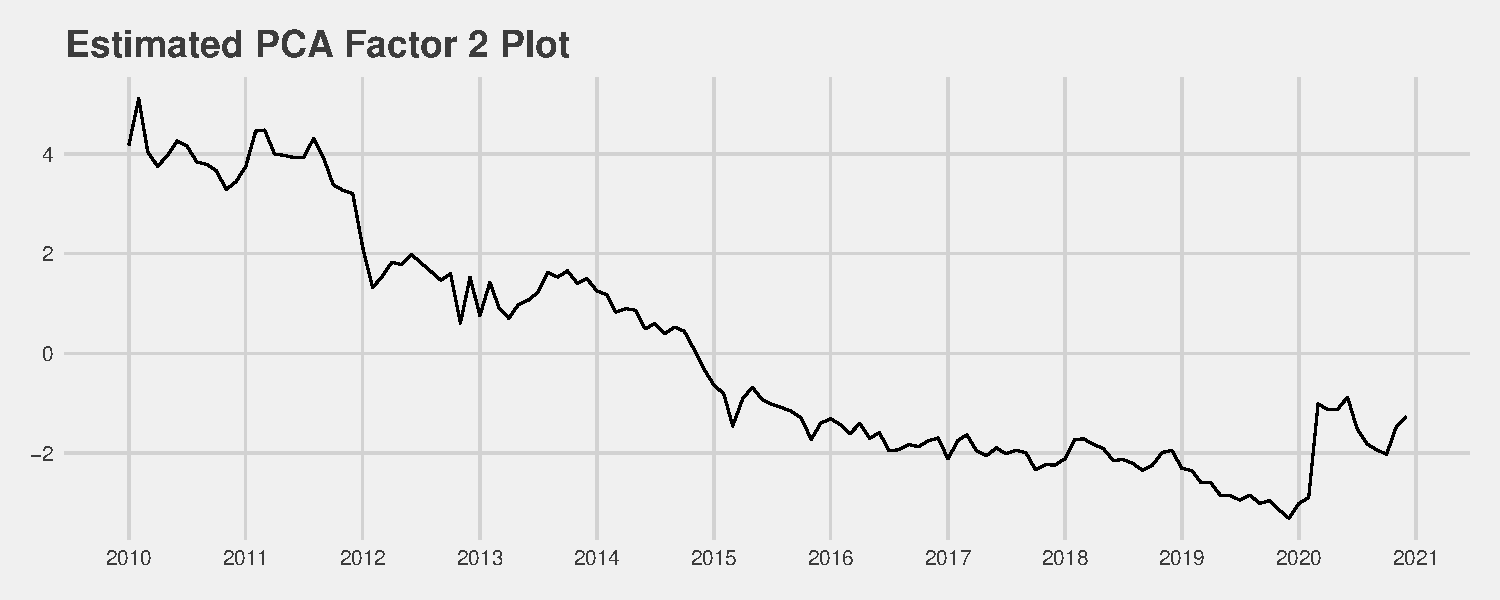
\includegraphics[width=5in,height=2in]{figure/unnamed-chunk-8-2} 

}




{\centering 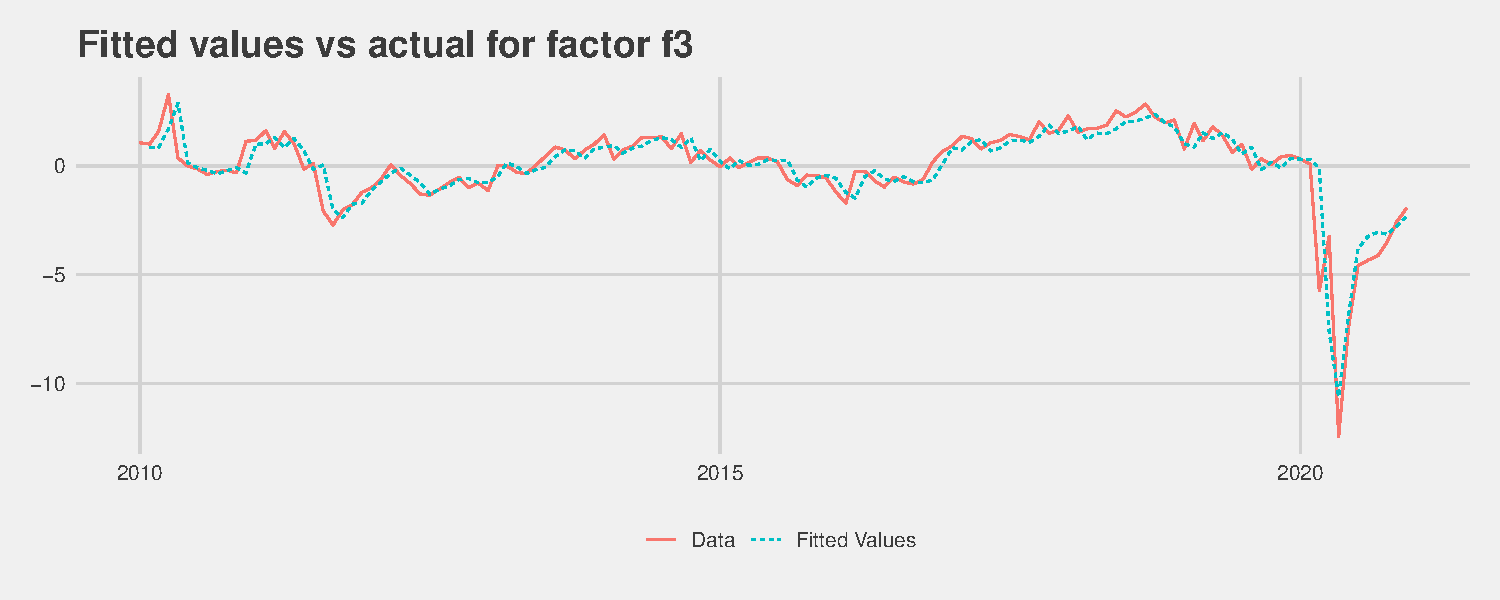
\includegraphics[width=5in,height=2in]{figure/unnamed-chunk-8-3} 

}







\subsection{Dynamic Factor Models}
Now let us consider again the monthly covariates which were include in the principal components analysis. We will model these as dynamic factor models (DFMs), i.e. - they are regressed on the factor variables derived from earlier.

The factor models take the following form:
\begin{align*}
\underbrace{\begin{bmatrix}
	\vv{ue}_t\\
	\vv{pce}_t\\
	\vdots \\
	\vv{claims}_t
\end{bmatrix}}_{y_t}
=
A
\underbrace{\begin{bmatrix}
	\vv{f1}_{t}\\
	\vv{f2}_{t}\\
	\vdots \\
	\vv{fR}_{t}
\end{bmatrix}}_{z_t}
+
\underbrace{\begin{bmatrix}
	w1_t\\
	w2_t\\
	\vdots\\
	wN_t
\end{bmatrix}}_{w_t},\\
\text{where $y_t$ is the $N \times 1$ vector of monthly variables at time $t$,}\\
\text{$A$ is the $N \times R$ coefficient matrix,}\\
\text{$z_t$ is the $R \times 1$ vector of factors at time $t$,}\\
\text{and $w_t$ is the $N \times 1$ vector of errors at time $t$.}\\
\end{align*}
We wish to estimate the coefficient matrix $A$. As before, we can do this by estimating this as an OLS equation, writing the data matrices as follows

\begin{equation}
\underbrace{\begin{bmatrix}
\vv{ue}_{2} & \vv{pce}_{2} & \dots & \vv{claims}_{2}\\
\vv{ue}_{3} & \vv{pce}_{3} & \dots & \vv{claims}_{3}\\
\vdots & \vdots & \vdots & \vdots \\
\vv{ue}_{T} & \vv{pce}_{T} & \dots & \vv{claims}_{T}\\
\end{bmatrix}}_{\Phi}
=
\underbrace{\begin{bmatrix}
\vv{f1}_{2} & \vv{f2}_{2} & \dots & \vv{f6}_{2}\\
\vv{f1}_{3} & \vv{f2}_{3} & \dots & \vv{f6}_{3}\\
\vdots & \vdots & \vdots & \vdots \\
\vv{f1}_{T} & \vv{f2}_{T} & \dots & \vv{f6}_{T}\\
\end{bmatrix}}_{\Omega}
A'
 +
\underbrace{\begin{bmatrix}
w1_2 & w2_2 & \dots & wR_2\\
w1_3 & w2_3 & \dots & wR_3\\
\vdots\\
w1_T & w2_T & \dots & wR_T\\
\end{bmatrix}}_{W}
\end{equation}

As before we can estimate $A$ with the standard OLS estimator.
\begin{align*}
\widehat{A}' = (\Omega' \Omega)^{-1} (\Omega'\Phi)
\end{align*}

Estimated coefficients are the in-sample goodness-of-fit are shown below.
% latex table generated in R 4.0.4 by xtable 1.8-4 package
% Fri Feb 26 20:28:00 2021
\begin{table}[!h]
\centering
\begingroup\footnotesize
\begin{tabular}{lrrr}
  \hline
name & f1 & f2 & f3 \\ 
  \hline
mpce & -0.01 & 0.00 & -0.00 \\ 
  mpceg & -0.01 & 0.00 & -0.00 \\ 
  mpcegd & -0.01 & 0.00 & -0.01 \\ 
  mpcegn & -0.00 & 0.00 & -0.00 \\ 
  mpces & -0.01 & 0.00 & -0.00 \\ 
  pid & 0.00 & -0.00 & 0.00 \\ 
  hpi & 0.00 & 0.00 & -0.00 \\ 
  ffr & -0.01 & 0.20 & 0.15 \\ 
  t10y & -0.04 & -0.14 & 0.26 \\ 
  t01y & -0.04 & -0.14 & 0.26 \\ 
  vsales & -0.17 & 0.76 & 0.34 \\ 
  ue & 0.04 & 0.00 & -0.00 \\ 
  wei & -0.16 & -0.30 & 0.95 \\ 
  spy & -0.00 & 0.00 & 0.00 \\ 
  vix & 0.92 & -0.81 & -2.24 \\ 
  loansre & 0.00 & 0.00 & 0.00 \\ 
  loanscc & -0.00 & -0.00 & 0.01 \\ 
  stlfsi & 0.10 & -0.02 & -0.15 \\ 
  usd & 0.36 & 4.24 & -0.86 \\ 
  uemean & -0.37 & -2.46 & 0.62 \\ 
  advsales & -0.01 & -0.00 & -0.00 \\ 
  kclfi & -0.04 & 0.42 & 0.15 \\ 
  csent & -0.01 & 0.53 & 0.29 \\ 
  ipi & -0.00 & -0.00 & -0.00 \\ 
  sny & -2.15 & -0.42 & 4.21 \\ 
  cfnai & -0.57 & 0.00 & -0.06 \\ 
   \hline
\end{tabular}
\endgroup
\caption{Estimated DFM Coefficients} 
\end{table}


% latex table generated in R 4.0.4 by xtable 1.8-4 package
% Fri Feb 26 20:28:00 2021
\begin{table}[!h]
\centering
\begingroup\footnotesize
\begin{tabular}{lrr}
  \hline
varname & MAE & MSE \\ 
  \hline
advsales & 0.00 & 0.00 \\ 
  cfnai & -0.07 & 0.23 \\ 
  csent & 99.78 & 9957.21 \\ 
  ffr & 0.59 & 0.60 \\ 
  hpi & 0.00 & 0.00 \\ 
  ipi & 0.00 & 0.00 \\ 
  kclfi & -0.48 & 0.30 \\ 
  loanscc & 0.01 & 0.00 \\ 
  loansre & 0.00 & 0.00 \\ 
  mpce & 0.00 & 0.00 \\ 
  mpceg & 0.00 & 0.00 \\ 
  mpcegd & 0.01 & 0.00 \\ 
  mpcegn & 0.00 & 0.00 \\ 
  mpces & 0.00 & 0.00 \\ 
  pid & 0.00 & 0.00 \\ 
  sny & 6.18 & 112.94 \\ 
  spy & 0.01 & 0.00 \\ 
  stlfsi & -0.26 & 0.19 \\ 
  t01y & 2.27 & 5.25 \\ 
  t10y & 2.27 & 5.25 \\ 
  ue & -0.00 & 0.00 \\ 
  uemean & 29.67 & 897.40 \\ 
  usd & 103.78 & 10790.48 \\ 
  vix & 17.97 & 340.06 \\ 
  vsales & 15.97 & 256.04 \\ 
  wei & 1.62 & 4.00 \\ 
   \hline
\end{tabular}
\endgroup
\caption{DFM Goodness of Fit} 
\end{table}






\subsection{State-Space Setup}
Now, combining our equations for the DFM and the VAR, we have the below system.
\begin{align*}
z_t = B z_{t-1} + Cx + v_t\\
y_t = A z_t + w_t
\end{align*}

This system is now fully specified and in state-space form. The first equation is our state (or transition) equation. The second equation is our measurement equation. 

We use our estimated values $B$, $C$, and $A$ calculated in our previous two sections. To run the Kalman Filter, we will want to create the actual data matrices for $z_t$ and $y_t$. $z_t$ can be constructed as before, using data for factors from time 1 through $T$. However, unlike in the previous two sections, we will want to create $y_t$ matrices not for just time periods 1 through $T$, but now for time periods $1$ through $\tau$. Elements in $y_t$ may be set to any value for missing observations; the process of Kalmam filtration will render this choice irrelevant.

Specifically, we construct the matrices below.
\begin{align*}
z_t
=
\begin{bmatrix}
	\vv{f1}_{t}\\
	\vv{f2}_{t}\\
	\vdots \\
	\vv{fR}_{t}
\end{bmatrix}, \forall t \in 1, \dots, T\\
y_t
=
\begin{bmatrix}
	\text{$\vv{ue}_{t}$ if available, otherwise 0}\\
	\text{$\vv{pce}_{t}$ if available, otherwise 0}\\
	\vdots \\
	\text{$\vv{claims}_{t}$ if available, otherwise 0}\\
\end{bmatrix}, \forall t \in 1, \dots, \tau
\end{align*}

For Kalman filtration, we also require an assumed distribution on $v_t$ and $w_t$. We assume that $v_t$ is distributed normally with mean 0 and constant diagonal covariance matrix denoted $Q$, with diagonal entries calculated by taking the average squared values of the residuals of the VAR.

We also assume $w_t$ is distributed normally with mean $0$. However, we no longer specify the covariance matrix as constant, but as the time-dependent matrices $R_t$. For $t \in 1, \dots, T+1$, we let $R_t$ be a diagonal covariance matrix with diagonal entries calcualted by taking the average squared values of the residuals of the DFM. For $t \in T+1, \dots, \tau$, we let the diagonal elements of $R_t$ be equal to infinity if the corresponding element of $y_t$ is missing for that time period; and equal to the average squared value of the residual if otherwise.
\begin{align*}
	v_t \sim \mathcal{N}(0, Q)\\
	w_t \sim \mathcal{N}(0, R_t)
\end{align*}

We begin with the unconditional mean of $\widehat{Z}_{0|-1} = 0$ and unconditional variance of VAR $\Sigma_{0|-1} = 0$.

\section{Kalman Filtration}
Now that our state-space model is fully specified, we can begin the Kalman filter recursions.
\begin{align*}
	z_t = B z_{t-1} + Cx + v_t\\
	y_t = A z_t + w_t\\
	v_t \sim \mathcal{N}(0, Q)\\
	w_t \sim \mathcal{N}(0, R_t)
\end{align*}

To solve this programmatically, we will need the previously estimated matrices $A$, $B$, and $C$; the matrices $z_t$ from 1 through $T$; the matrices $y_t$ from 1 through $\tau$; the covariance matrix $Q$; and finally, the covariance matrices $R_t$ from 1 through $\tau$.

We initialize the Kalman filter with the following standard assumptions. 
\begin{align*}
	\vv{z}_{0|0} = 0\\
	\vv{CovZ} = 0
\end{align*}

Now for $t = 1, \dots, \tau$, we iterate through the Kalman filter recursions and iteratively calculate the values below.
\begin{align*}
	\vv{z}_{t|t-1} &= B \vv{z}_{t-1|t-1} + C\\
	\vv{CovZ}_{t|t-1} &= B \vv{CovZ}_{t-1|t-1} + Q\\
	\vv{y}_{t|t-1} &= A \vv{z}_{t|t-1}\\
	\vv{CovY}_{t|t-1} &= A \vv{CovZ}_{t|t-1} A' + R_t\\
	P_t &= \vv{CovZ}_{t|t-1} A' \vv{CovY}^{-1}_{t|t-1}\\
	\vv{z}_{t|t} &= \vv{z}_{t|t-1} + P_t (\vv{y}_t - \vv{y}_{t|t-1})\\
	\vv{CovZ}_{t|t} &= \vv{CovZ}_{t|t-1} - P_t (\vv{CovY}_{t|t-1}) P'_t
\end{align*}
Note that the during recursions $T + 1, \dots \tau$, the infinite values in the $R_t$ matrix will cause infinite values in the $\vv{CovY}_{t|t-1}$ matrix. This may prevent standard computational methods from computing the inverse of the matrix needed in the step for calculation of $\vv{CovZ}_{t|t}$. Alternative methods, such as a Cholesky decomposition before inversion, can be used to subvert this problem.

The Kalman filter allows us to recover all the time $t$ conditional state matrices $z_{t|t}$ that have been adjusted for information from the monthly datasets. However, of more interest to us is the value of the state matrices when conditioned on all data available at time $\tau$, $z_{t|\tau}$. This can be recovered by using the Kalman smoother.

Recursively iterating over $t = \tau - 1, \dots, 1$, we calculate the following values. 
\begin{align*}
	S_{t} &= \vv{CovZ}_{t|t} B' \vv{CovZ}^{-1}_{t + 1|t}\\
	\vv{z}_{t|\tau} &= \vv{z}_{t|t} + S_t (\vv{z}_{t+1|\tau} - \vv{z}_{t + 1|t})\\
	\vv{CovZ}_{t|\tau} &= \vv{CovZ}_{t|t} - S_t(\vv{CovZ}_{t + 1|t} - \vv{CovZ}_{t + 1|\tau})S'_t
\end{align*}
These values $\vv{z}_{t|\tau}$ will serve as our estimates of the state variables (i.e., the PCA factors) from time 1 through $\tau$.

Finally, we want to forecast the the state vector $z_{t|\tau}$ for $t = \tau + 1, \dots, T^*$. This can be done through the typical Kalman filter forecasting step.

Recursively iterating over $t = \tau + 1, \dots, T^*$, we calculate the following values.
\begin{align*}
	\vv{z}_{t|\tau} &= B \vv{z}_{t-1|\tau} + C\\
	\vv{CovZ}_{t|\tau} &= B \vv{CovZ}_{t-1|\tau} B'+ Q\\
	\vv{y}_{t|\tau} &= A \vv{z}_{t|\tau}\\
	\vv{CovY}_{t|\tau} &= A \vv{CovZ}_{t|\tau} A' + R_0
\end{align*}
Combining the calculations for $\vv{z}_{t|\tau}$ with the ones derived from the Kalman smoother, we will now be able to obtain the full time series for the factors from time 1 through time $T^*$.



{\centering 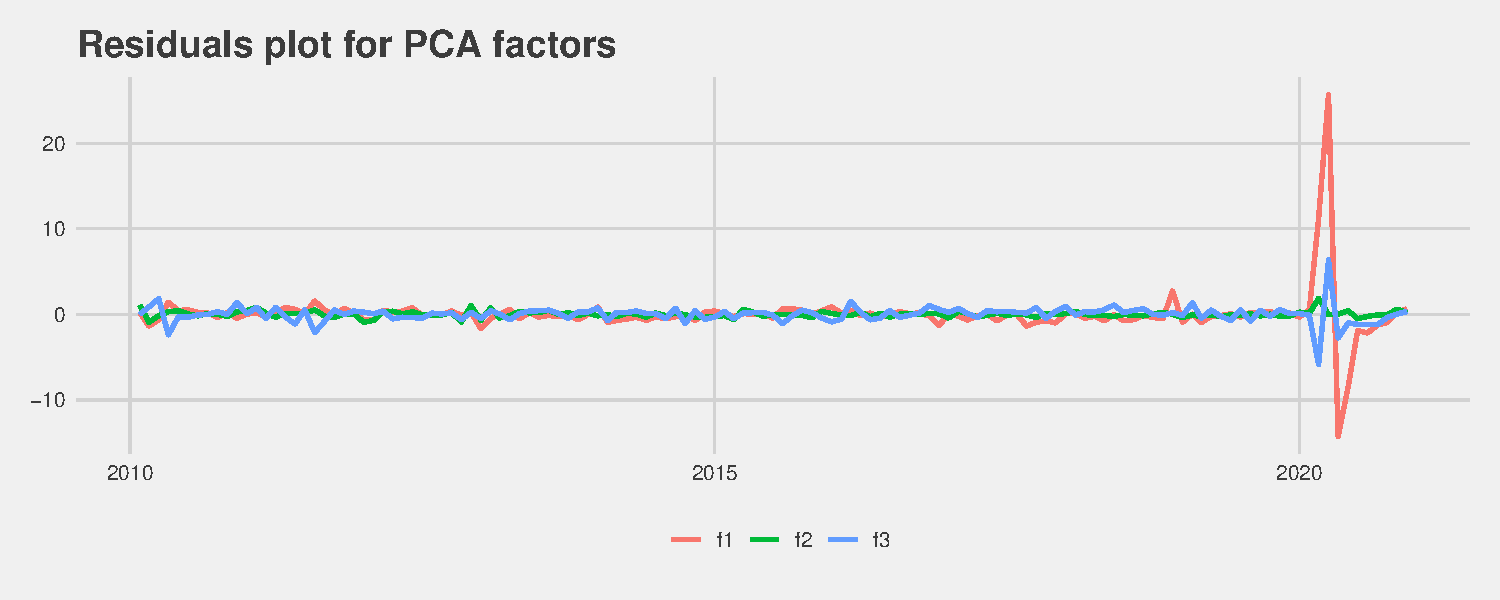
\includegraphics[width=5in,height=2in]{figure/unnamed-chunk-11-1} 

}




{\centering 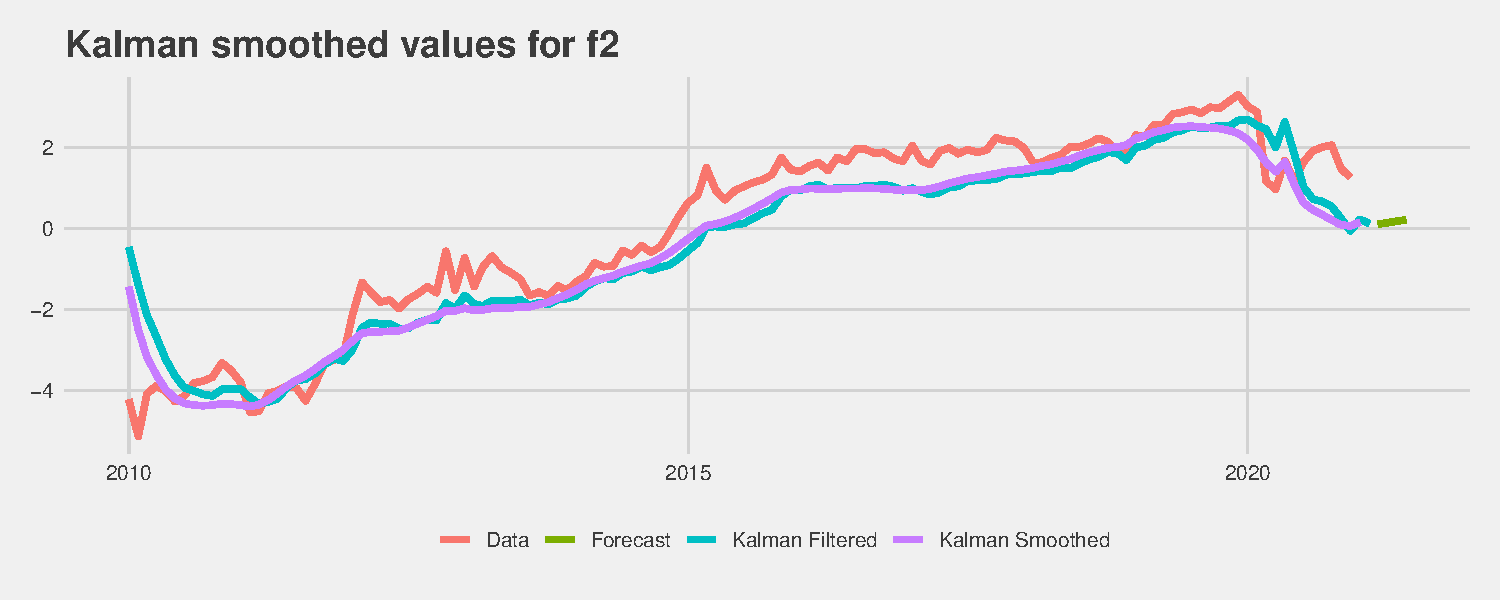
\includegraphics[width=5in,height=2in]{figure/unnamed-chunk-11-2} 

}




{\centering 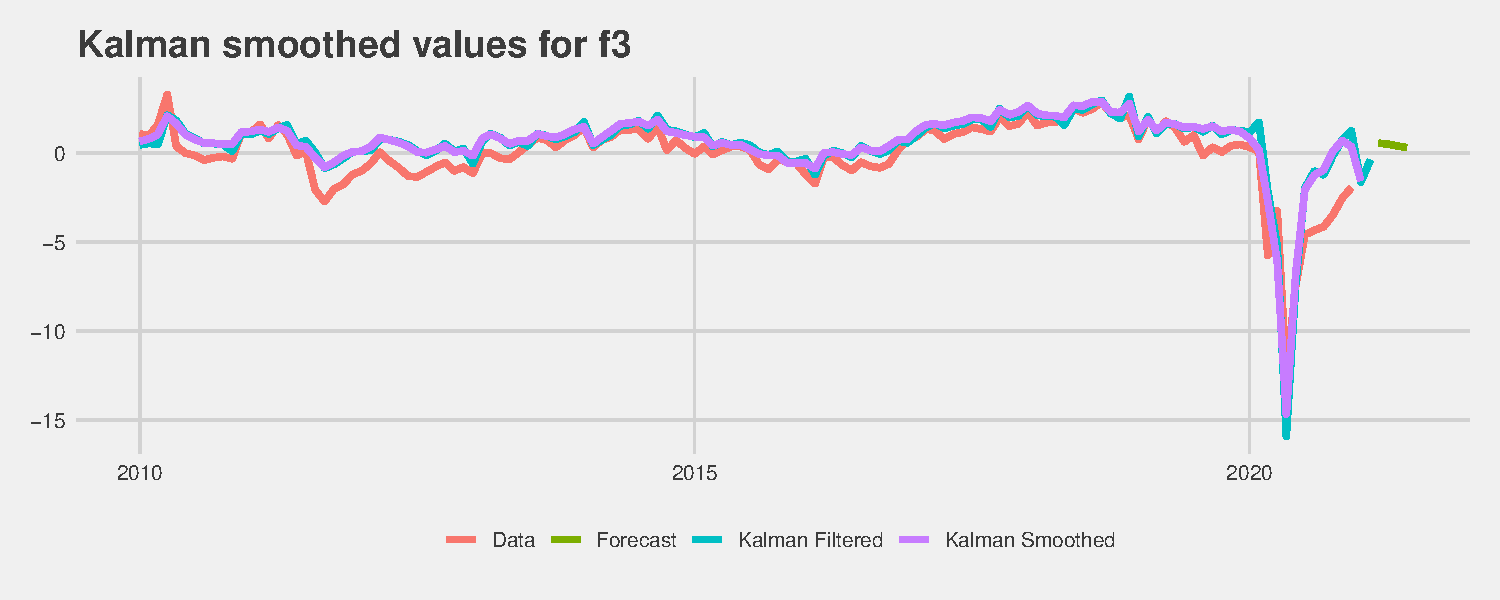
\includegraphics[width=5in,height=2in]{figure/unnamed-chunk-11-3} 

}





\section{Predicting GDP}
Now that we have the smoothed factor values, we can use these in the dynamic factor model to nowcast our variables of interest.

Work in progress...



\end{document}
